\documentclass[aspectratio=169,10pt]{beamer}

% ==========================================================================
% NVIDIA-style theme (custom, no external theme package required)
% ==========================================================================

% ==== Packages ====
\usepackage[utf8]{inputenc}
\usepackage[T1]{fontenc}
\usepackage{lmodern}
\usepackage{helvet}            % Helvetica-like sans-serif (close to NVIDIA Sans)
\renewcommand{\familydefault}{\sfdefault}
\usepackage{textcomp}
\usepackage{amssymb}
\usepackage{listings}
\usepackage{xcolor}
\usepackage{booktabs}
\usepackage{array}
\usepackage{tikz}
\usepackage{hyperref}
\usepackage[absolute,overlay]{textpos}
\usetikzlibrary{arrows.meta,positioning,shapes.geometric,fit,calc,backgrounds}

% ==== NVIDIA color palette (from sample.pptx theme1.xml) ====
\definecolor{nvgreen}{HTML}{76B900}        % primary brand green
\definecolor{nvgreendark}{HTML}{5A8F00}
\definecolor{nvblack}{HTML}{000000}
\definecolor{nvgray}{HTML}{5E5E5E}
\definecolor{nvgraylt}{HTML}{8C8C8C}
\definecolor{nvcaption}{HTML}{CDCDCD}
\definecolor{nvbgalt}{HTML}{F4F4F4}        % soft cream/gray for content boxes
\definecolor{nvblue}{HTML}{0071C5}         % accent blue (from palette)
\definecolor{nvteal}{HTML}{008564}         % accent teal
\definecolor{nvpurple}{HTML}{5D1682}       % accent purple
\definecolor{nvmagenta}{HTML}{890C58}      % accent magenta

% ==== Back-compat color aliases (slides body refers to slblue/slgreen/etc.) ====
\colorlet{slgreen}{nvgreen}                % map green accents to NVIDIA green
\colorlet{slblue}{nvblue}
\colorlet{slred}{nvmagenta}
\colorlet{sloran}{nvteal}

% ==== Code listing colors ====
\definecolor{codebg}{HTML}{F4F4F4}
\definecolor{codekw}{HTML}{76B900}         % keywords in NVIDIA green
\definecolor{codestr}{HTML}{890C58}        % strings in magenta
\definecolor{codecom}{HTML}{5E5E5E}        % comments in gray
\definecolor{codeln}{HTML}{8C8C8C}

% ==== Beamer surface colors ====
\setbeamercolor{normal text}{fg=nvblack,bg=white}
\setbeamercolor{structure}{fg=nvgreen}
\setbeamercolor{frametitle}{fg=nvblack,bg=white}
\setbeamercolor{title}{fg=white}
\setbeamercolor{alerted text}{fg=nvgreen}
\setbeamercolor{itemize item}{fg=nvgreen}
\setbeamercolor{itemize subitem}{fg=nvgreen}
\setbeamercolor{itemize subsubitem}{fg=nvgreen}
\setbeamercolor{enumerate item}{fg=nvgreen}
\setbeamercolor{block title}{fg=white,bg=nvgreen}
\setbeamercolor{block body}{fg=nvblack,bg=nvbgalt}
\setbeamercolor{caption name}{fg=nvgray}
\setbeamercolor{section in toc}{fg=nvblack}
\setbeamercolor{subsection in toc}{fg=nvgray}

\setbeamerfont{frametitle}{size=\Large,series=\bfseries}
\setbeamerfont{title}{size=\huge,series=\bfseries}
\setbeamerfont{block title}{size=\normalsize,series=\bfseries}

% ==== Remove clutter ====
\setbeamertemplate{navigation symbols}{}

% Auto-insert a section divider slide at the start of every \section
\AtBeginSection[]{%
  {\setbeamercolor{background canvas}{bg=nvblack}%
   \begin{frame}[plain]
     \sectionpage
   \end{frame}%
  }%
}

% ==== Frame title: bold black, green accent underline + small NVIDIA logo top-right ====
\setbeamertemplate{frametitle}{%
  \nointerlineskip%
  \vspace*{0.4cm}%
  \hspace*{0.6cm}\begin{minipage}[t]{\dimexpr\paperwidth-4.0cm\relax}%
    \raggedright%
    \strut\insertframetitle\strut\\[-0.1em]%
    {\color{nvgreen}\rule{2.2em}{2.6pt}}%
  \end{minipage}%
  % Logo floating in top-right corner of the frame (only on non-title slides)
  \begin{textblock*}{2cm}(13.6cm,0.35cm)
    \includegraphics[height=0.5cm]{nvidia_logo.png}%
  \end{textblock*}%
}

% ==== Headline / footline ====
\setbeamertemplate{headline}{}
\setbeamertemplate{footline}{%
  \hspace*{0.6cm}{\footnotesize\color{nvgray}\insertshorttitle}%
  \hfill%
  {\footnotesize\color{nvgray}\insertframenumber\,/\,\inserttotalframenumber}\hspace*{0.6cm}%
  \vspace{0.25cm}%
}

% ==== Section page: full-bleed NVIDIA green swoosh background ====
\setbeamertemplate{section page}{%
  \begin{tikzpicture}[remember picture, overlay]
    % Full-bleed background image (image3.jpg: green swoosh)
    \node[anchor=south west,inner sep=0pt] at (current page.south west)
      {
\includegraphics[width=\paperwidth,height=\paperheight]{nv_section_bg.jpg}};
    % Thin vertical green bar at the far left
    \fill[nvgreen] (current page.north west) rectangle
      ($(current page.south west)+(3mm,0)$);
    % Section title at top-left (matches layoutLayout230 placement)
    \node[anchor=north west,text width=14cm,align=left]
      at ($(current page.north west)+(0.8cm,-1.0cm)$)
      {{\color{nvgreen}\rule{2.2em}{2.6pt}}\\[0.5em]%
       {\color{nvblack}\LARGE\bfseries\insertsection}};
  \end{tikzpicture}%
}

% ==== Custom title page: NVIDIA keynote-style full-bleed "glow eye" bg ====
\setbeamertemplate{title page}{%
  \begin{tikzpicture}[remember picture, overlay]
    % Full-bleed background image (image42.png: glowing NVIDIA eye on black)
    \node[anchor=south west,inner sep=0pt] at (current page.south west)
      {\includegraphics[width=\paperwidth,height=\paperheight]{nv_title_bg.png}};
    % NVIDIA logo top-left (matches layoutLayout166 placement)
    \node[anchor=north west]
      at ($(current page.north west)+(0.5cm,-0.7cm)$)
      {\includegraphics[height=0.85cm]{nvidia_logo.png}};
    % Title block bottom-left
    \node[anchor=south west,text width=\paperwidth,inner sep=0pt]
      at ($(current page.south west)+(0.8cm,1.2cm)$)
      {{\color{nvgreen}\rule{3.5em}{3pt}}\\[0.6em]%
       {\color{white}\Huge\bfseries\inserttitle}\\[0.4em]%
       {\color{nvcaption}\Large\insertsubtitle}\\[1em]%
       {\color{nvgraylt}\small\insertdate}};
  \end{tikzpicture}%
}

% ==== Custom agenda / outline page (image6 on left, content on right) ====
% The sample PPTX places the green-swoosh image at (0,0) with width=4.69 of 10 slide-units
% and dimensions 4.69x5.62 (i.e. covers the left ~47% and the full height).
% We reproduce that by fixing both width and height for the background image.
\newcommand{\agendapage}[2]{% #1 = title, #2 = content
  \begin{tikzpicture}[remember picture, overlay]
    % Left image, clipped to the left 47% of the slide (width x full height) ----
    \node[anchor=north west,inner sep=0pt]
      at (current page.north west)
      {
\includegraphics[width=7.5cm,height=\paperheight]{nv_agenda_bg.jpg}};
    % White overlay to ensure the right-half is pure white (defensive)
    \fill[white] ($(current page.north west)+(7.55cm,0)$)
                 rectangle (current page.south east);
    % Vertical green divider (thin accent)
    \fill[nvgreen] ($(current page.north west)+(7.4cm,-3mm)$)
       rectangle ($(current page.south west)+(7.55cm,3mm)$);
    % Title on the right
    \node[anchor=north west,text width=7.8cm]
      at ($(current page.north west)+(7.9cm,-1.0cm)$)
      {{\color{nvblack}\Large\bfseries #1}\\[0.2em]%
       {\color{nvgreen}\rule{2.2em}{2.6pt}}\\[0.9em]%
       #2};
  \end{tikzpicture}%
}

% ==== Listings config for Python (NVIDIA-green keywords on off-white bg) ====
\lstdefinestyle{py}{
  language=Python,
  backgroundcolor=\color{codebg},
  basicstyle=\ttfamily\tiny,
  keywordstyle=\color{codekw}\bfseries,
  stringstyle=\color{codestr},
  commentstyle=\color{codecom}\itshape,
  numbers=left,
  numberstyle=\color{codeln}\tiny,
  numbersep=5pt,
  frame=leftline,
  framesep=4pt,
  rulecolor=\color{nvgreen},
  framerule=1.5pt,
  breaklines=true,
  showstringspaces=false,
  tabsize=4,
  xleftmargin=12pt,
  aboveskip=4pt,
  belowskip=4pt,
}
\lstset{style=py}

% Hyperlink colors
\hypersetup{
  colorlinks=true,
  urlcolor=nvgreen,
  linkcolor=nvgreen,
}

% ==== Meta ====
\title[SGLang + Helix]{[ACOT] SGLang --- Helix Parallelism}
\subtitle{Knowledge Sharing}
\author{}
\institute{}
\date{\today}

\begin{document}

% ========= TITLE =========
\begin{frame}[plain]
  \titlepage
\end{frame}

% ========= AGENDA (outline) =========
\begin{frame}[plain]
  \agendapage{Agenda}{%
    \scriptsize
    \begin{itemize}\itemsep2pt
      \item \textbf{Process topology} --- HTTP, Scheduler, Detokenizer, the two communication planes
      \item \textbf{Attention backends} --- FlashInfer / FA3 / FA4 / Triton via Strategy pattern
      \item \textbf{CUDA graphs} --- capture, bucket-based replay, backend hooks
      \item \textbf{Parallelism} --- TP / PP / DP input preparation and inter-layer data flow
      \item \textbf{Communication} --- NCCL, PyNCCL, CustomAllreduce, symmetric memory
      \item \textbf{End-to-end request flow} --- HTTP $\to$ tokens $\to$ stream
      \item \textbf{Case study: Helix parallelism} --- DCP + TPA + A2A (MLA and GQA)
    \end{itemize}%
    \vspace{0.3cm}\par%
    \color{nvgray}All code paths under \texttt{python/sglang/srt/}.%
  }
\end{frame}

% =========================================================================
\section{Process topology}
% =========================================================================

\begin{frame}{SGLang is a constellation of processes}
  \begin{columns}[T,onlytextwidth]
    \begin{column}{0.55\textwidth}
      \begin{center}
        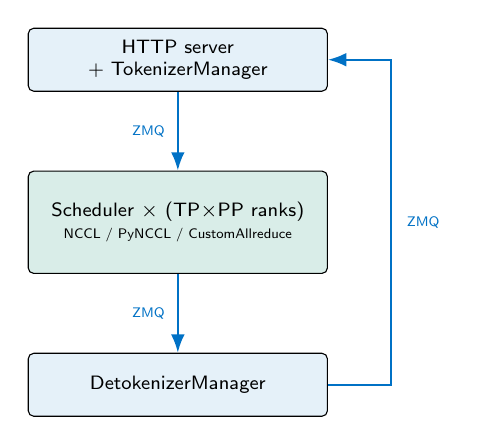
\begin{tikzpicture}[node distance=0.6cm, font=\scriptsize]
          \tikzstyle{box}=[draw,rounded corners=2pt,minimum width=3.8cm,minimum height=0.8cm,align=center,fill=slblue!10]
          \tikzstyle{sbox}=[draw,rounded corners=2pt,minimum width=3.8cm,minimum height=1.3cm,align=center,fill=sloran!15]
          \node[box] (http) {HTTP server\\ + TokenizerManager};
          \node[sbox,below=1.0cm of http] (sched) {Scheduler $\times$ (TP$\times$PP ranks)\\{\tiny NCCL / PyNCCL / CustomAllreduce}};
          \node[box,below=1.0cm of sched] (detok) {DetokenizerManager};
          % Downward data-plane arrows (left lane)
          \draw[-{Latex},thick,slblue] (http.south) -- node[left,xshift=-1pt]{\tiny ZMQ} (sched.north);
          \draw[-{Latex},thick,slblue] (sched.south) -- node[left,xshift=-1pt]{\tiny ZMQ} (detok.north);
          % Return arrow (right rail) --- L-shaped, fully outside the boxes
          \draw[-{Latex},thick,slblue]
            (detok.east) -- ++(0.8,0) |-
            node[pos=0.25,right,xshift=2pt]{\tiny ZMQ}
            (http.east);
        \end{tikzpicture}
      \end{center}
    \end{column}
    \begin{column}{0.42\textwidth}
      \footnotesize
      Two transports, two planes:
      \begin{itemize}
        \item \textcolor{slblue}{\textbf{ZMQ IPC}} between CPU processes (requests, token IDs, strings)
        \item \textcolor{slred}{\textbf{NCCL}} between GPU processes in the same TP/PP/MoE group (collectives inside one forward)
      \end{itemize}
      \vspace{0.2cm}
      The Scheduler cluster is the only place NCCL is used. Everything crossing a CPU boundary rides ZMQ.
    \end{column}
  \end{columns}
\end{frame}

\begin{frame}{Control plane vs data plane}
  \centering
  \small
  \begin{tabular}{p{3.5cm} p{5.2cm} p{4.3cm}}
    \toprule
    \textbf{Plane} & \textbf{Transport} & \textbf{What travels} \\
    \midrule
    Control & \textcolor{slblue}{ZMQ IPC} (PUSH/PULL, pickled Python) & Requests, token IDs, strings \\[2pt]
    Data    & \textcolor{slred}{NCCL / PyNCCL / CustomAllreduce / symm mem} & Hidden states, KV, expert acts \\
    \bottomrule
  \end{tabular}
  \vspace{0.5cm}
  \begin{itemize}\footnotesize
    \item HTTP $\to$ TokenizerManager $\to$ Scheduler $\to$ Detokenizer --- all ZMQ.
    \item Inside a forward pass (all-reduce, all-to-all, PP send/recv) --- all NCCL.
    \item Detokenizer never touches NCCL --- it holds no GPU state.
  \end{itemize}
\end{frame}

% =========================================================================
\section{Attention backends}
% =========================================================================

\begin{frame}{Attention backends --- 15+ kernels, one interface}
  \begin{columns}[T,onlytextwidth]
    \begin{column}{0.55\textwidth}
      \footnotesize
      Supported backends (subset):
      \begin{itemize}\scriptsize
        \item FlashInfer / FlashInfer-MLA
        \item FlashAttention~3 and~4 (same class!)
        \item Triton / DoubleSparse
        \item FlashMLA, TRT-LLM MLA, cuDNN
        \item Native Sparse, Aiter (AMD), Wave, Ascend NPU
        \item Intel AMX / XPU, TorchNative, FlexAttention
      \end{itemize}
      \vspace{0.2cm}
      All of them implement one ABC:
      \begin{center}\texttt{AttentionBackend}\end{center}
    \end{column}
    \begin{column}{0.45\textwidth}
      \centering
      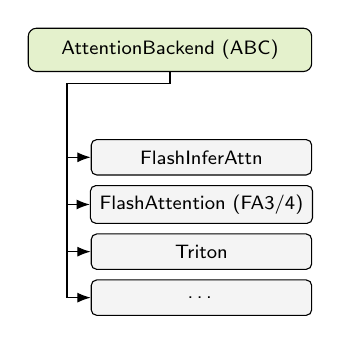
\begin{tikzpicture}[node distance=0.12cm,font=\scriptsize]
        \tikzstyle{abc}=[draw,rounded corners=3pt,minimum width=3.6cm,minimum height=0.55cm,align=center,fill=slgreen!20]
        \tikzstyle{cc}=[draw,rounded corners=2pt,minimum width=2.8cm,minimum height=0.45cm,fill=codebg]
        \node[abc] (a) {AttentionBackend (ABC)};
        \node[cc,below=0.85cm of a.south,xshift=0.4cm] (fi) {FlashInferAttn};
        \node[cc,below=0.12cm of fi]              (fa) {FlashAttention (FA3/4)};
        \node[cc,below=0.12cm of fa]              (tr) {Triton};
        \node[cc,below=0.12cm of tr]              (al) {\dots};
        % Spine for UML-style tree
        \coordinate (top)  at ($(a.south)+(0,-0.15)$);
        \coordinate (tl)   at ($(fi.west)+(-0.3,0)$);
        \coordinate (bl)   at ($(al.west)+(-0.3,0)$);
        \draw (a.south) -- (top) -| (tl);
        \draw (tl) -- (bl);
        \draw[-{Latex}] (tl |- fi.west) -- (fi.west);
        \draw[-{Latex}] (tl |- fa.west) -- (fa.west);
        \draw[-{Latex}] (tl |- tr.west) -- (tr.west);
        \draw[-{Latex}] (tl |- al.west) -- (al.west);
      \end{tikzpicture}
    \end{column}
  \end{columns}
\end{frame}

\begin{frame}[fragile]{Strategy + Template Method}
  \footnotesize
  \texttt{python/sglang/srt/layers/attention/base\_attn\_backend.py:80--123} --- the ABC's \texttt{forward} is the template method:
\begin{lstlisting}
@debug_kernel_api
def forward(self, q, k, v, layer, forward_batch, save_kv_cache=True, **kwargs):
    if forward_batch.forward_mode.is_idle():
        return q.new_empty(q.shape[0], layer.tp_q_head_num * layer.v_head_dim)
    elif forward_batch.forward_mode.is_decode():
        return self.forward_decode(q, k, v, layer, forward_batch,
                                    save_kv_cache=save_kv_cache, **kwargs)
    elif forward_batch.forward_mode.is_mixed() and is_npu():
        return self.forward_mixed(...)
    else:
        return self.forward_extend(q, k, v, layer, forward_batch,
                                    save_kv_cache=save_kv_cache, **kwargs)
\end{lstlisting}
  \vspace{-0.2cm}
  \begin{itemize}\scriptsize
    \item Only \texttt{init\_forward\_metadata} is truly abstract.
    \item Subclasses only override \texttt{forward\_decode} / \texttt{forward\_extend}.
    \item The dispatch policy lives in one place, so backends can't disagree.
  \end{itemize}
\end{frame}

\begin{frame}[fragile]{Registry + Factory --- Open/Closed Principle}
  \footnotesize
  \texttt{python/sglang/srt/layers/attention/attention\_registry.py} --- decorator-based plugin table:
\begin{lstlisting}
ATTENTION_BACKENDS = {}

def register_attention_backend(name):
    def decorator(fn):
        ATTENTION_BACKENDS[name] = fn
        return fn
    return decorator

@register_attention_backend("flashinfer")
def create_flashinfer_backend(runner):
    if not runner.use_mla_backend:
        from sglang.srt.layers.attention.flashinfer_backend import FlashInferAttnBackend
        return FlashInferAttnBackend(runner, init_new_workspace=runner.init_new_workspace)
    ...
\end{lstlisting}
  \begin{itemize}\scriptsize
    \item Adding a new backend = one decorated function; no changes to existing code.
    \item \texttt{ModelRunner} does \texttt{ATTENTION\_BACKENDS[name](self)} to build it.
  \end{itemize}
\end{frame}

\begin{frame}[fragile]{Dependency injection --- no \texttt{if} in the model}
  \footnotesize
  \texttt{python/sglang/srt/layers/radix\_attention.py:133--170}:
\begin{lstlisting}
def forward(self, q, k, v, forward_batch, save_kv_cache=True, **kwargs):
    ...
    ret = forward_batch.attn_backend.forward(
        q, k, v, self, forward_batch, save_kv_cache, **kwargs,
    )
    return self._maybe_slice_output_heads(ret)
\end{lstlisting}
  \vspace{0.2cm}
  \begin{block}{What's \emph{not} here}
    \small
    No \texttt{if backend == "flashinfer"\dots elif\dots} anywhere.\\
    The backend is injected once (via \texttt{ForwardBatch}) and flows through every layer.
  \end{block}
\end{frame}

% =========================================================================
\section{CUDA graphs}
% =========================================================================

\begin{frame}{CUDA graphs --- why}
  \begin{columns}[T,onlytextwidth]
    \begin{column}{0.55\textwidth}
      \footnotesize
      Decoding launches \emph{thousands} of tiny kernels per token:
      \begin{itemize}\scriptsize
        \item Per-layer: 4--6 kernels (QKV, attn, O, gate\_up, activation, down).
        \item $\times$ \emph{L} layers = 100--500 kernels per step.
        \item Each launch adds $\sim 5\,\mu s$ of host latency.
      \end{itemize}
      \vspace{0.3cm}
      \textbf{Fix:} record them once into a CUDA graph, then \texttt{graph.replay()} --- a \emph{single} driver call launches the whole sequence.
      \vspace{0.3cm}
      Works only when shapes are fixed $\Rightarrow$ one graph per batch-size bucket.
    \end{column}
    \begin{column}{0.42\textwidth}
      \centering
      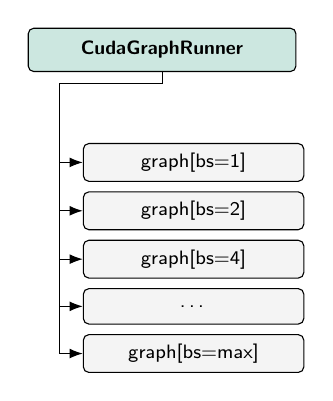
\begin{tikzpicture}[font=\scriptsize,node distance=0.12cm]
        \tikzstyle{b}=[draw,rounded corners=2pt,minimum width=3.4cm,minimum height=0.55cm,align=center,fill=sloran!20]
        \tikzstyle{sb}=[draw,rounded corners=2pt,minimum width=2.8cm,minimum height=0.45cm,fill=codebg]
        \node[b] (c) {\textbf{CudaGraphRunner}};
        \node[sb,below=0.9cm of c.south,xshift=0.4cm] (g1) {graph[bs=1]};
        \node[sb,below=0.12cm of g1] (g2) {graph[bs=2]};
        \node[sb,below=0.12cm of g2] (g4) {graph[bs=4]};
        \node[sb,below=0.12cm of g4] (gd) {\dots};
        \node[sb,below=0.12cm of gd] (gn) {graph[bs=max]};
        % Spine-and-branches layout (no line crosses a box)
        \coordinate (top) at ($(c.south)+(0,-0.15)$);
        \coordinate (tl)  at ($(g1.west)+(-0.3,0)$);
        \coordinate (bl)  at ($(gn.west)+(-0.3,0)$);
        \draw (c.south) -- (top) -| (tl);
        \draw (tl) -- (bl);
        \draw[-{Latex}] (tl |- g1.west) -- (g1.west);
        \draw[-{Latex}] (tl |- g2.west) -- (g2.west);
        \draw[-{Latex}] (tl |- g4.west) -- (g4.west);
        \draw[-{Latex}] (tl |- gd.west) -- (gd.west);
        \draw[-{Latex}] (tl |- gn.west) -- (gn.west);
      \end{tikzpicture}
    \end{column}
  \end{columns}
\end{frame}

\begin{frame}[fragile]{Capture loop --- large $\to$ small for pool reuse}
  \footnotesize
  \texttt{python/sglang/srt/model\_executor/cuda\_graph\_runner.py:855--871}:
\begin{lstlisting}
# Trigger CUDA graph capture for specific shapes.
# Capture the large shapes first so that the smaller shapes
# can reuse the memory pool allocated for the large shapes.
with freeze_gc(self.model_runner.server_args.enable_cudagraph_gc):
    if not self.enable_pdmux:
        with graph_capture() as graph_capture_context, profile_context as prof:
            self.stream = graph_capture_context.stream
            _capture_one_stream()
    else:
        for i, sg in enumerate(self.stream_groups):
            with graph_capture(stream=sg[1]) as graph_capture_context, profile_context as prof:
                self.stream = graph_capture_context.stream
                _capture_one_stream(i)
\end{lstlisting}
  \begin{itemize}\scriptsize
    \item \texttt{graph\_capture()} is a context manager from \texttt{python/sglang/srt/distributed/parallel\_state.py} --- puts TP/PP/MoE groups in a graph-safe mode.
    \item Each bucket gets \texttt{torch.cuda.CUDAGraph.capture\_begin/\_end} around \texttt{model.forward}.
    \item \texttt{CUDAGraph.pool\_handle()} is reused so buckets share memory.
  \end{itemize}
\end{frame}

\begin{frame}[fragile]{Replay --- bucket lookup + buffer copy}
  \footnotesize
  \texttt{python/sglang/srt/model\_executor/cuda\_graph\_runner.py:1279--1308}:
\begin{lstlisting}
def replay(self, forward_batch, skip_attn_backend_init=False, pp_proxy_tensors=None):
    self.deepep_adapter.replay()

    if not skip_attn_backend_init:
        self.replay_prepare(forward_batch, pp_proxy_tensors)
    else:
        self.buffers.input_ids[:self.raw_num_token].copy_(forward_batch.input_ids)
        self.buffers.positions[:self.raw_num_token].copy_(forward_batch.positions)
        ...

    # Replay
    graph_key = self.bs
    self.graphs[graph_key].replay()
    output = self.output_buffers[graph_key]
\end{lstlisting}
  \vspace{-0.2cm}
  Three steps: copy inputs into fixed buffers $\to$ refresh attention metadata $\to$ \texttt{graph.replay()}.
\end{frame}

\begin{frame}[fragile]{Graph dispatch in ModelRunner}
  \footnotesize
  \texttt{python/sglang/srt/model\_executor/model\_runner.py:3115--3146}:
\begin{lstlisting}
mode_check = (forward_batch.forward_mode.is_cpu_graph
              if self.device == "cpu"
              else forward_batch.forward_mode.is_cuda_graph)
can_run_graph = bool(mode_check()
                     and self.graph_runner
                     and self.graph_runner.can_run(forward_batch))
...
if can_run_graph:
    ret = self.graph_runner.replay(
        forward_batch,
        skip_attn_backend_init=skip_attn_backend_init,
        pp_proxy_tensors=pp_proxy_tensors,
    )
    return ModelRunnerOutput(logits_output=ret, can_run_graph=can_run_graph)
\end{lstlisting}
  \begin{itemize}\scriptsize
    \item Eligible modes: \texttt{DECODE}, \texttt{TARGET\_VERIFY}, \texttt{IDLE}, \texttt{DLLM\_EXTEND}.
    \item Prefill / extend normally takes the eager path (variable seq lens).
  \end{itemize}
\end{frame}

% =========================================================================
\section{Parallelism}
% =========================================================================

\begin{frame}{Parallelism axes in SGLang --- we focus on TP}
  \centering
  \small
  \begin{tabular}{l p{9cm}}
    \toprule
    \textbf{Axis} & \textbf{What it shards} \\
    \midrule
    \textbf{TP} \textcolor{slred}{(focus)} & \textbf{Weights (heads / channels) --- all ranks see same tokens} \\
    PP & Layers --- each rank owns a contiguous layer range \\
    DP (replicas) & Independent model replicas; different requests per replica \\
    DP-attention & Same model, different \emph{tokens} per DP rank (for KV cache scaling) \\
    EP & MoE experts --- different experts on different ranks \\
    CP / DCP & Sequence / KV dimension for long contexts \\
    \bottomrule
  \end{tabular}
  \vspace{0.4cm}
  \footnotesize
  TP is the canonical axis --- the rest follow the same pattern.\\
  The key design lesson: \textcolor{slred}{\textbf{the model code never calls NCCL directly}} --- it only talks to \texttt{tp\_group}.
\end{frame}

\begin{frame}[fragile]{The TP abstraction --- model talks to \texttt{tp\_group}, not NCCL}
  \footnotesize
  The entire model-visible communication API (\texttt{python/sglang/srt/distributed/communication\_op.py}):
\begin{lstlisting}
def tensor_model_parallel_all_reduce(x):
    return get_tp_group().all_reduce(x)

def tensor_model_parallel_all_gather(x, dim=-1):
    return get_tp_group().all_gather(x, dim)

def tensor_model_parallel_reduce_scatter(x, dim=0):
    return get_tp_group().reduce_scatter(x, dim)
\end{lstlisting}
  \vspace{-0.15cm}
  \texttt{get\_tp\_group()} returns a \texttt{GroupCoordinator} with these methods:
  \begin{center}\scriptsize
  \begin{tabular}{l p{7cm}}
    \toprule
    \texttt{tp\_group.all\_reduce(x)}          & sum across ranks; every rank gets the sum \\
    \texttt{tp\_group.all\_gather(x, dim)}     & concat slices from every rank \\
    \texttt{tp\_group.reduce\_scatter(x, dim)} & sum then scatter, each rank keeps a slice \\
    \texttt{tp\_group.broadcast(x, src)}       & one rank sends \texttt{x} to every other rank \\
    \bottomrule
  \end{tabular}
  \end{center}
  \vspace{0.2cm}
  \begin{block}{Key point}\small
    NCCL / PyNccl / CustomAllreduce / symmetric memory / mscclpp are picked \emph{inside}
    \texttt{GroupCoordinator} --- \textbf{the model layer doesn't know any of them exist}.
  \end{block}
\end{frame}

\begin{frame}[fragile]{TP groups --- consecutive ranks}
  \footnotesize
  \texttt{python/sglang/srt/distributed/parallel\_state.py:1872--1893}:
\begin{lstlisting}
# Build the tensor model-parallel groups.
num_tensor_model_parallel_groups = world_size // tensor_model_parallel_size
group_ranks = []
for tp_group_idx in range(num_tensor_model_parallel_groups):
    ranks = list(range(
        tp_group_idx * tensor_model_parallel_size,
        (tp_group_idx + 1) * tensor_model_parallel_size,
    ))
    group_ranks.append(ranks)

_TP = init_model_parallel_group(
    group_ranks, get_world_group().local_rank, backend,
    use_message_queue_broadcaster=envs.SGLANG_USE_MESSAGE_QUEUE_BROADCASTER.get(),
    group_name="tp",
)
\end{lstlisting}
  \begin{itemize}\scriptsize
    \item Each \texttt{GroupCoordinator} wraps \emph{two} \texttt{ProcessGroup}s: NCCL (device) + gloo (CPU).
    \item CPU group is used for broadcasting pickled Python objects.
  \end{itemize}
\end{frame}

\begin{frame}[fragile]{Parallel linear layers --- the building blocks}
  \footnotesize
  \begin{columns}[T,onlytextwidth]
    \begin{column}{0.48\textwidth}
      \scriptsize
      \texttt{layers/linear.py}:
      \vspace{0.2cm}
      \begin{itemize}
        \item \texttt{ColumnParallelLinear} --- shards weight on \emph{output} dim; emits partial output.
        \item \texttt{MergedColumnParallelLinear} --- several column-parallel stacked (gate\_up).
        \item \texttt{QKVParallelLinear} --- column-parallel, head-aware (GQA support).
        \item \texttt{RowParallelLinear} --- shards weight on \emph{input} dim; all-reduces output to full.
        \item \texttt{VocabParallelEmbedding} --- vocab dim sharded; all-reduces.
      \end{itemize}
    \end{column}
    \begin{column}{0.48\textwidth}
      \scriptsize
      \textbf{Invariant contract:}\\[2pt]
      \begin{tabular}{@{}lll@{}}
        \toprule
        Layer & Output & Comm \\
        \midrule
        Col-parallel & partial & \textcolor{slgreen}{none} \\
        Row-parallel & full & \textcolor{slred}{all-reduce} \\
        Vocab-embed  & full & \textcolor{slred}{all-reduce} \\
        RadixAttn    & partial & \textcolor{slgreen}{none} \\
        RMSNorm / SiLU & any & \textcolor{slgreen}{none} \\
        \bottomrule
      \end{tabular}
      \vspace{0.2cm}
      Col-parallel $\to$ \dots $\to$ Row-parallel = one all-reduce, hidden inside.
    \end{column}
  \end{columns}
\end{frame}

\begin{frame}[fragile]{\texttt{RowParallelLinear.forward} --- the hidden all-reduce}
  \footnotesize
\begin{lstlisting}
def forward(self, input_, skip_all_reduce=False):
    if self.input_is_parallel:
        input_parallel = input_
    else:
        splitted_input = split_tensor_along_last_dim(input_, self.tp_size)
        input_parallel = splitted_input[self.tp_rank].contiguous()

    # Matrix multiply.
    # Only fuse bias add into GEMM for rank 0 (avoid bias * tp_size)
    bias_ = None if (self.tp_rank > 0 or self.skip_bias_add) else self.bias
    with symm_ctx:
        output_parallel = self.quant_method.apply(self, input_parallel, bias=bias_)

    if self.reduce_results and self.tp_size > 1 and not skip_all_reduce:
        output = tensor_model_parallel_all_reduce(output_parallel)   # <- ALL-REDUCE
    else:
        output = output_parallel
    return output, (self.bias if self.skip_bias_add else None)
\end{lstlisting}
  \begin{itemize}\scriptsize
    \item Bias trick: only rank 0 adds bias; all-reduce then gives correct $b$ exactly once.
    \item \texttt{self.quant\_method.apply} runs the actual GEMM (FP16, FP8, GPTQ, AWQ, \dots).
  \end{itemize}
\end{frame}

\begin{frame}[fragile]{Llama --- no explicit collective calls}
  \footnotesize
  \texttt{python/sglang/srt/models/llama.py} --- \texttt{LlamaAttention}:
\begin{lstlisting}
self.qkv_proj = QKVParallelLinear(...)       # column-parallel
self.o_proj   = RowParallelLinear(...)       # row-parallel (all-reduce)

def forward(self, positions, hidden_states, forward_batch):
    qkv, _ = self.qkv_proj(hidden_states)
    q, k, v = qkv.split([self.q_size, self.kv_size, self.kv_size], dim=-1)
    q, k = self.rotary_emb(positions, q, k)
    attn_output = self.attn(q, k, v, forward_batch)
    output, _ = self.o_proj(attn_output)     # <- all-reduce happens inside
    return output
\end{lstlisting}
  \begin{block}{Key insight}
    \small
    The model \emph{never} calls \texttt{torch.distributed.*}. Communication is encoded by the
    \emph{choice of layer type}.
  \end{block}
\end{frame}

\begin{frame}{Data flow through one Llama decoder layer, TP$=4$}
  \centering
  \tiny
  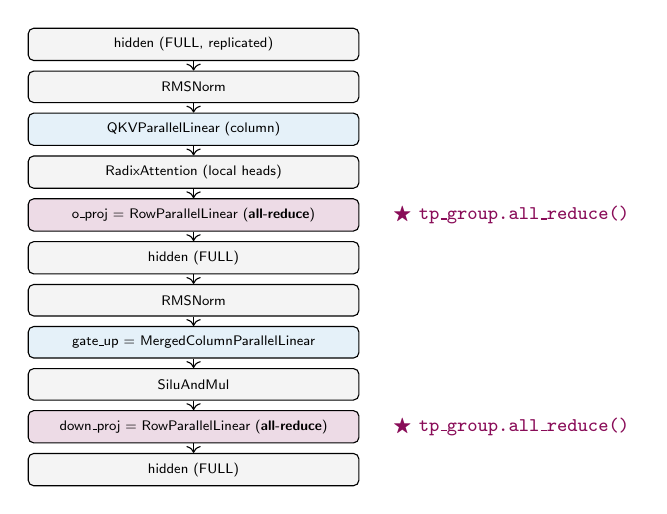
\begin{tikzpicture}[node distance=0.12cm,font=\tiny]
    \tikzstyle{b}=[draw,rounded corners=2pt,minimum width=4.2cm,minimum height=0.4cm,fill=codebg]
    \tikzstyle{c}=[draw,rounded corners=2pt,minimum width=4.2cm,minimum height=0.4cm,fill=slblue!10]
    \tikzstyle{r}=[draw,rounded corners=2pt,minimum width=4.2cm,minimum height=0.4cm,fill=slred!15]
    \node[b] (h0)   {hidden (FULL, replicated)};
    \node[b,below=of h0]   (n1) {RMSNorm};
    \node[c,below=of n1]   (qkv) {QKVParallelLinear (column)};
    \node[b,below=of qkv]  (att) {RadixAttention (local heads)};
    \node[r,below=of att]  (op)  {o\_proj = RowParallelLinear (\textbf{all-reduce})};
    \node[b,below=of op]   (h1)  {hidden (FULL)};
    \node[b,below=of h1]   (n2)  {RMSNorm};
    \node[c,below=of n2]   (gu)  {gate\_up = MergedColumnParallelLinear};
    \node[b,below=of gu]   (si)  {SiluAndMul};
    \node[r,below=of si]   (dp)  {down\_proj = RowParallelLinear (\textbf{all-reduce})};
    \node[b,below=of dp]   (h2)  {hidden (FULL)};
    \draw[->] (h0) -- (n1);
    \draw[->] (n1) -- (qkv);
    \draw[->] (qkv) -- (att);
    \draw[->] (att) -- (op);
    \draw[->] (op) -- (h1);
    \draw[->] (h1) -- (n2);
    \draw[->] (n2) -- (gu);
    \draw[->] (gu) -- (si);
    \draw[->] (si) -- (dp);
    \draw[->] (dp) -- (h2);
    \node[right=0.3cm of op,text=slred,font=\scriptsize]  {$\bigstar$ \texttt{tp\_group.all\_reduce()}};
    \node[right=0.3cm of dp,text=slred,font=\scriptsize]  {$\bigstar$ \texttt{tp\_group.all\_reduce()}};
  \end{tikzpicture}\\
  Two all-reduces per transformer block $\Rightarrow$ $2L$ for an $L$-layer model.
\end{frame}

\begin{frame}[fragile]{TP input --- same batch, broadcast via gloo}
  \footnotesize
  \texttt{python/sglang/srt/managers/scheduler.py:1584--1590}:
\begin{lstlisting}
elif self.tp_size != 1:
    recv_reqs = broadcast_pyobj(
        recv_reqs,
        self.tp_group.rank,
        self.tp_cpu_group,            # <- gloo CPU group
        src=self.tp_group.ranks[0],
    )
\end{lstlisting}
  \begin{itemize}\small
    \item Rank 0 pulls requests from ZMQ.
    \item CPU-side gloo broadcast ships pickled Python objects to every TP rank.
    \item Every rank then builds an identical \texttt{ForwardBatch} and runs in lockstep.
  \end{itemize}
\end{frame}

% =========================================================================
\section{Communication}
% =========================================================================

\begin{frame}[fragile]{\texttt{GroupCoordinator.all\_reduce} --- picks the fastest path}
  \footnotesize
\begin{lstlisting}
def all_reduce(self, input_):
    if self.world_size == 1:
        return input_
    ...
    # 1. Symm-mem pynccl (fast when available)
    if self.pynccl_comm is not None and self.is_symmetric_memory_enabled():
        with self.pynccl_comm.change_state(enable=True):
            self.pynccl_comm.all_reduce(input_)
            return input_

    # 2. Size/mode-dependent outplace paths
    outplace_all_reduce_method = None
    if self.ca_comm and self.ca_comm.should_custom_ar(input_):
        outplace_all_reduce_method = "ca"
    elif self.qr_comm and self.qr_comm.should_quick_allreduce(input_):
        outplace_all_reduce_method = "qr"
    elif self.pymscclpp_comm and self.pymscclpp_comm.should_mscclpp_allreduce(input_):
        outplace_all_reduce_method = "pymscclpp"
    elif is_in_piecewise_cuda_graph() and self.pynccl_comm is not None:
        outplace_all_reduce_method = "pynccl"
    if outplace_all_reduce_method is not None:
        return outplace_all_reduce(input_, group_name=self.unique_name,
                                   outplace_all_reduce_method=outplace_all_reduce_method)

    # 3. Fallback: inplace PyNccl or torch.distributed
    inplace_all_reduce(input_, group_name=self.unique_name)
    return input_
\end{lstlisting}
\end{frame}

\begin{frame}{Why so many all-reduce variants?}
  \footnotesize
  \begin{tabular}{p{3cm} p{9.2cm}}
    \toprule
    \textbf{Variant} & \textbf{When it wins} \\
    \midrule
    \texttt{CustomAllreduce}    & Small tensors, no graph --- IPC one-shot / two-shot \\
    \texttt{QuickAllreduce}     & AMD with symmetric memory \\
    \texttt{pymscclpp}          & Medium-size tensors; MSCCL++ topology-aware \\
    \texttt{TorchSymmMem}       & PyTorch symmetric memory --- peer P2P reads \\
    \texttt{PyNccl}             & Any size, works \emph{inside} a CUDA graph \\
    \texttt{torch.distributed}  & Universal fallback \\
    \bottomrule
  \end{tabular}
  \vspace{0.4cm}
  \begin{block}{Takeaway}
    \small
    The fastest primitive depends on tensor size, group size, hardware, and whether a CUDA graph
    is being captured. One policy, centralized in \texttt{GroupCoordinator}, picks the best per call.
  \end{block}
\end{frame}

% =========================================================================
\section{End-to-end flow}
% =========================================================================

\begin{frame}[fragile]{HTTP $\to$ TokenizerManager $\to$ SSE}
  \footnotesize
  \texttt{python/sglang/srt/entrypoints/http\_server.py:689--718}:
\begin{lstlisting}
async def generate_request(obj: GenerateReqInput, request: Request):
    if obj.stream:
        async def stream_results() -> AsyncIterator[bytes]:
            async for out in _global_state.tokenizer_manager.generate_request(obj, request):
                yield b"data: " + dumps_json(out) + b"\n\n"
            yield b"data: [DONE]\n\n"
        return StreamingResponse(
            stream_results(),
            media_type="text/event-stream",
            background=_global_state.tokenizer_manager.create_abort_task(obj),
        )
    else:
        ret = await _global_state.tokenizer_manager.generate_request(obj, request).__anext__()
        return orjson_response(ret)
\end{lstlisting}
  OpenAI endpoints (\texttt{/v1/chat/completions}) go through Pydantic validation first, then land on the same \texttt{generate\_request}.
\end{frame}

\begin{frame}[fragile]{Scheduler main loop}
  \footnotesize
  \texttt{python/sglang/srt/managers/scheduler.py:1382--1407}:
\begin{lstlisting}
def event_loop_normal(self):
    """A normal scheduler loop."""
    while True:
        recv_reqs = self.recv_requests()         # ZMQ + broadcast_pyobj
        self.process_input_requests(recv_reqs)   # -> waiting_queue
        ...
        batch = self.get_next_batch_to_run()     # prefill or decode
        self.cur_batch = batch
        if batch:
            result = self.run_batch(batch)       # -> model_worker.forward_batch_generation
            self.process_batch_result(batch, result)  # -> detokenizer
\end{lstlisting}
  \begin{itemize}\scriptsize
    \item \texttt{get\_next\_batch\_to\_run} does RadixCache prefix-lookup and batch formation.
    \item \texttt{run\_batch} delegates to \texttt{TpModelWorker}, which drives \texttt{ModelRunner.forward}.
  \end{itemize}
\end{frame}

\begin{frame}{Output chain --- logits, then tokens, then strings}
  \centering
  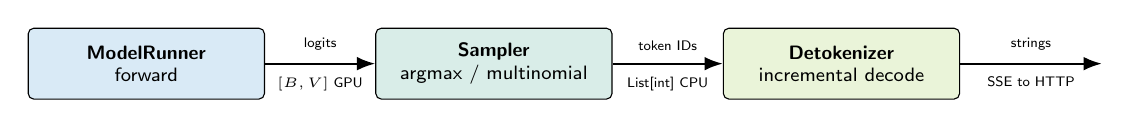
\begin{tikzpicture}[node distance=1.4cm,font=\scriptsize]
    \tikzstyle{b}=[draw,rounded corners=2pt,minimum width=3.0cm,minimum height=0.9cm,align=center,fill=codebg]
    \node[b,fill=slblue!15]               (m) {\textbf{ModelRunner}\\forward};
    \node[b,fill=sloran!15,right=of m]    (s) {\textbf{Sampler}\\argmax / multinomial};
    \node[b,fill=slgreen!15,right=of s]   (d) {\textbf{Detokenizer}\\incremental decode};
    \coordinate[right=1.8cm of d] (dend);
    \draw[-{Latex},thick] (m) -- node[above=1pt,font=\tiny]{logits}
                                node[below=1pt,font=\tiny]{$[B,V]$ GPU} (s);
    \draw[-{Latex},thick] (s) -- node[above=1pt,font=\tiny]{token IDs}
                                node[below=1pt,font=\tiny]{List[int] CPU} (d);
    \draw[-{Latex},thick] (d.east) -- node[above=1pt,font=\tiny]{strings}
                                     node[below=1pt,font=\tiny]{SSE to HTTP} (dend);
  \end{tikzpicture}
  \vspace{0.4cm}
  \begin{itemize}\footnotesize
    \item \texttt{ModelRunner.forward} returns \texttt{LogitsProcessorOutput.next\_token\_logits} --- raw logits, not probabilities.
    \item \texttt{ModelRunner.sample} runs \texttt{Sampler.forward} --- argmax (greedy) or multinomial (top-k/top-p).
    \item Detokenizer is a separate process, ZMQ-connected. No NCCL in this chain.
  \end{itemize}
\end{frame}

\begin{frame}{End-to-end timeline (one decode step)}
  \footnotesize
  \begin{enumerate}\itemsep2pt
    \item Client POSTs \texttt{/v1/chat/completions} $\rightarrow$ FastAPI handler (HTTP server).
    \item \texttt{TokenizerManager} tokenizes the prompt, assigns a \texttt{rid}, sends \texttt{TokenizedGenerateReqInput} to Scheduler via \textcolor{slblue}{\textbf{ZMQ PUSH}}.
    \item Scheduler rank 0 pulls the request; \texttt{broadcast\_pyobj} (gloo) replicates it to every TP rank.
    \item Scheduler calls \texttt{ModelRunner.forward} $\Rightarrow$ \texttt{ForwardBatch} runs through the transformer;\\
          $2L$ \textcolor{slred}{\textbf{NCCL}} all-reduces happen \emph{inside} the parallel linear layers.
    \item Last PP rank runs \texttt{Sampler} to produce token IDs.
    \item Scheduler pushes \texttt{BatchTokenIDOutput} to \texttt{DetokenizerManager} via \textcolor{slblue}{\textbf{ZMQ PUSH}}.
    \item Detokenizer does incremental HF decoding, pushes \texttt{BatchStrOutput} back to \texttt{TokenizerManager}.
    \item \texttt{TokenizerManager} wakes the per-\texttt{rid} asyncio event; the HTTP handler emits an SSE chunk.
  \end{enumerate}
  \vspace{0.3cm}
  \centering\footnotesize Prefill runs once; decode repeats steps 3--8 once per output token until the stop condition.
\end{frame}

% =========================================================================
\section{Case study: Helix parallelism}
% =========================================================================

\begin{frame}{Helix --- the KV duplication problem}
  \footnotesize
  \textbf{Standard TP fails when \texttt{tp\_size > num\_kv\_heads}.}

  For MLA (1 effective KV head) at \texttt{tp=8} the KV cache is \emph{replicated} 8$\times$
  --- erasing MLA's memory savings at long context.

  \vspace{0.4cm}
  \begin{tabular}{lccc}
    \toprule
    Model & KV heads & TP=8 dup & TP=16 dup \\
    \midrule
    Llama-3 405B (GQA-8) & 8   & 1$\times$ & 2$\times$ \\
    Nemotron-49B (GQA-8) & 8   & 1$\times$ & 2$\times$ \\
    DeepSeek-V2/V3/R1 (MLA) & 1 eff. & \textcolor{slred}{\textbf{8$\times$}} & \textcolor{slred}{\textbf{16$\times$}} \\
    \bottomrule
  \end{tabular}

  \vspace{0.4cm}
  \textbf{Helix} (NVIDIA, July 2025) decouples attention from FFN:
  \[
    \boxed{\texttt{tp\_size} = \underbrace{\texttt{tpa\_size}}_{\text{head shard}}
                             \times \underbrace{\texttt{dcp\_size}}_{\text{KV-seq shard}}}
    \qquad \text{with}\quad \texttt{tpa\_size} \le \texttt{num\_kv\_heads}
  \]

  Result on DeepSeek-V2, 1M context, 8$\times$H100: \textcolor{slred}{\textbf{25.5 ms $\to$ 7.3 ms TPOT (−71\%)}}.
\end{frame}

\begin{frame}{Helix in numbers --- 32 Q heads, 4 KV heads, sequence S, TP=8}
  \scriptsize
  \begin{columns}[T,onlytextwidth]
    % ============================ LEFT: PLAIN TP=8 ============================
    \begin{column}{0.49\textwidth}
      \textbf{Plain TP=8} (KV cache duplicated)\\[0.2em]
      Each GPU gets 4 Q heads + 1 KV head + \emph{full} S.\\
      With only 4 KV heads, neighbor pairs hold the \textbf{same} KV.

      \vspace{0.3em}
      \begin{tabular}{@{}clll@{}}
        \toprule
        GPU & Q heads & KV head & Seq \\
        \midrule
        0 & Q[0--3]   & KV[0]                                & S \\
        1 & Q[4--7]   & \textcolor{slred}{KV[0] (dup of GPU0)} & S \\
        2 & Q[8--11]  & KV[1]                                & S \\
        3 & Q[12--15] & \textcolor{slred}{KV[1] (dup of GPU2)} & S \\
        4 & Q[16--19] & KV[2]                                & S \\
        5 & Q[20--23] & \textcolor{slred}{KV[2] (dup of GPU4)} & S \\
        6 & Q[24--27] & KV[3]                                & S \\
        7 & Q[28--31] & \textcolor{slred}{KV[3] (dup of GPU6)} & S \\
        \bottomrule
      \end{tabular}

      \vspace{0.4em}
      \textbf{KV memory:} per-GPU $S\!\times\!1\!\times\!d$, total $\mathbf{8S\!\times\!d}$ \\
      Useful $4S\!\times\!d$ $\Rightarrow$ \textcolor{slred}{\textbf{50\% wasted to duplication}}.
    \end{column}

    % ============================ RIGHT: HELIX DCP=2 ==========================
    \begin{column}{0.49\textwidth}
      \textbf{TP=8 with TPA=4 $\times$ DCP=2} (Helix --- no duplication)\\[0.2em]
      Each GPU gets 8 Q heads + 1 KV head + \emph{half} S.\\
      Pair (GPU0,1) shares the same heads but split the sequence.

      \vspace{0.3em}
      \begin{tabular}{@{}clll@{}}
        \toprule
        GPU & Q heads & KV head & Seq \\
        \midrule
        0 & Q[0--7]   & KV[0] & S/2 (first half)  \\
        1 & Q[0--7]   & KV[0] & S/2 (second half) \\
        2 & Q[8--15]  & KV[1] & S/2 (first half)  \\
        3 & Q[8--15]  & KV[1] & S/2 (second half) \\
        4 & Q[16--23] & KV[2] & S/2 (first half)  \\
        5 & Q[16--23] & KV[2] & S/2 (second half) \\
        6 & Q[24--31] & KV[3] & S/2 (first half)  \\
        7 & Q[24--31] & KV[3] & S/2 (second half) \\
        \bottomrule
      \end{tabular}

      \vspace{0.4em}
      \textbf{KV memory:} per-GPU $\tfrac{S}{2}\!\times\!1\!\times\!d$, total $\mathbf{4S\!\times\!d}$ \\
      Equals exactly the natural KV cache size $\Rightarrow$ \textcolor{slgreen}{\textbf{0\% duplication}}.

      \vspace{0.4em}
      \textbf{Two new groups:} \texttt{attn\_tp\_group} = \{0,2,4,6\}, \{1,3,5,7\}; \texttt{dcp\_group} = \{0,1\}, \{2,3\}, \{4,5\}, \{6,7\}.
    \end{column}
  \end{columns}
\end{frame}

\begin{frame}{Helix = DCP + TPA + A2A}
  \footnotesize
  \begin{columns}[T,onlytextwidth]
    \begin{column}{0.48\textwidth}
      \textbf{DCP (Decode Context Parallelism)}
      \begin{itemize}\scriptsize
        \item Shard KV cache across ranks by token position (interleaved: \texttt{pos \% dcp\_size}).
        \item Each rank runs attention on its local KV shard and returns \emph{partial} output + LSE.
      \end{itemize}
      \vspace{0.2cm}
      \textbf{TPA (Tensor Parallel Attention)}
      \begin{itemize}\scriptsize
        \item Constrained head-shard: \texttt{tpa\_size $\le$ num\_kv\_heads}.
        \item MLP stays full-TP --- so TPA + DCP = full TP.
      \end{itemize}
      \vspace{0.2cm}
      \textbf{A2A (All-to-All reduction)}
      \begin{itemize}\scriptsize
        \item Replaces AG(Q) + AG(O) + RS with 2 all-to-alls.
        \item Exact softmax merge via LSE-weighted combine.
      \end{itemize}
    \end{column}
    \begin{column}{0.48\textwidth}
      \textbf{Two flavors I implemented}
      \begin{center}\scriptsize
      \begin{tabular}{l l}
        \toprule
        Flavor & Formula \\
        \midrule
        \textbf{MLA Helix}  & \texttt{dcp + a2a}        \\
        \textbf{GQA Helix}  & \texttt{dcp + tpa + a2a}  \\
        \bottomrule
      \end{tabular}
      \end{center}
      \vspace{0.3cm}
      \textbf{Why "layered"}: both flavors only add\\
      (i) one new \textcolor{slblue}{\textbf{group}} (\texttt{\_DCP}, \texttt{\_ATTN\_TP}),\\
      (ii) one new \textcolor{slred}{\textbf{kernel}} (\texttt{dcp\_a2a\_lse\_reduce}),\\
      (iii) one new \textcolor{slgreen}{\textbf{branch}} in the attention backend and the model code.\\[0.2cm]
      Nothing else in SGLang changes.
    \end{column}
  \end{columns}
\end{frame}

\begin{frame}{MLA Helix (DCP + A2A) --- SGLang core paths modified}
  \footnotesize
  \begin{enumerate}\itemsep3pt
    \item \textbf{Scheduler / KV allocator --- each rank gets only its slice of token slots.}\\
          \texttt{python/sglang/srt/mem\_cache/allocator.py :: TokenToKVPoolAllocator.alloc}:
          \vspace{-0.1cm}
          \begin{center}\scriptsize
          \texttt{local\_mask = (token\_positions \% dcp\_world\_size) == dcp\_rank}
          \end{center}
          The scheduler passes \texttt{token\_positions} so the rank knows which tokens it owns.
    \item \textbf{Per-layer local page table} --- new helper in \texttt{python/sglang/srt/layers/attention/dcp\_layout.py} maps\\
          \textit{global} token positions $\to$ \textit{local} page IDs this rank holds.\\
          Every attention backend now takes the \emph{local} page table instead of the global one.
    \item \textbf{New collective: \texttt{dcp\_a2a\_lse\_reduce}} --- new file \texttt{python/sglang/srt/layers/attention/dcp\_a2a.py}.\\
          Triton pack $\to$ 2$\times$ \texttt{dcp\_group.all\_to\_all\_single} $\to$ Triton LSE-weighted merge.\\
          Replaces 3 NCCL calls with 2.
    \item \textbf{Attention backend contract} --- FA3 / FlashInfer MLA \texttt{forward\_decode} now returns\\
          \texttt{(output, lse)} when \texttt{use\_dcp}; \textbf{model} then calls \texttt{dcp\_a2a\_lse\_reduce}.
    \item \textbf{Model (\texttt{python/sglang/srt/models/deepseek\_common/attention\_forward\_methods/forward\_mla.py})} --- all-gather Q across DCP, run attention on local KV, LSE-combine,\\
          then continue into \texttt{o\_proj} as normal.
  \end{enumerate}
\end{frame}

\begin{frame}{GQA Helix (DCP + TPA + A2A) --- additional modifications}
  \footnotesize
  All of the MLA changes, plus four more touch points because GQA models have $>1$ KV heads and
  we want to shard them across a \emph{separate} attention-TP group:

  \begin{enumerate}\itemsep3pt
    \item \textbf{New process group \texttt{\_ATTN\_TP}} --- \texttt{python/sglang/srt/distributed/parallel\_state.py}.\\
          Accessors: \texttt{get\_attention\_tp\_group()}, \texttt{get\_attention\_tp\_rank()},
          \texttt{get\_attention\_tp\_size()}.
    \item \textbf{Weight loading with TPA} --- \texttt{qkv\_proj} / \texttt{o\_proj} now pass \emph{attention-TP}
          rank+size to \texttt{QKVParallelLinear} / \texttt{RowParallelLinear}:
          \vspace{-0.05cm}
          \begin{center}\scriptsize
            \texttt{QKVParallelLinear(..., tp\_rank=get\_attention\_tp\_rank(),}
            \texttt{tp\_size=get\_attention\_tp\_size())}
          \end{center}
          MLP weights still shard across full TP.
    \item \textbf{TPA $\to$ full-TP handoff} --- \texttt{python/sglang/srt/layers/communicator.py}: \texttt{use\_full\_tp\_attention\_handoff}.\\
          \texttt{o\_proj} has \texttt{reduce\_results=False}; communicator does the \emph{full-TP} all-reduce
          that sums over both the TPA head slice and the residual.
    \item \textbf{Model wiring} (\texttt{python/sglang/srt/models/qwen3\_moe.py}, \texttt{python/sglang/srt/models/qwen2.py}) --- \texttt{attn\_for\_dcp\_decode} with a wider
          \texttt{RadixAttention} of \texttt{num\_heads $\times$ dcp\_size} Q heads, all-gather Q over DCP, A2A combine.
  \end{enumerate}
\end{frame}

\begin{frame}{Attention block under GQA Helix (TP=8, TPA=4, DCP=2)}
  \centering
  \scriptsize
  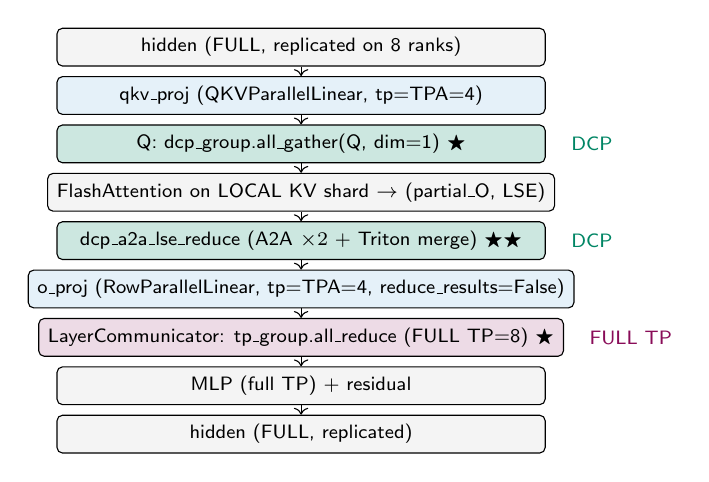
\begin{tikzpicture}[node distance=0.12cm,font=\scriptsize]
    \tikzstyle{b}=[draw,rounded corners=2pt,minimum width=6.2cm,minimum height=0.45cm,fill=codebg]
    \tikzstyle{c}=[draw,rounded corners=2pt,minimum width=6.2cm,minimum height=0.45cm,fill=slblue!10]
    \tikzstyle{dcp}=[draw,rounded corners=2pt,minimum width=6.2cm,minimum height=0.45cm,fill=sloran!20]
    \tikzstyle{fulltp}=[draw,rounded corners=2pt,minimum width=6.2cm,minimum height=0.45cm,fill=slred!15]
    \node[b] (h0)   {hidden (FULL, replicated on 8 ranks)};
    \node[c,below=of h0]   (qkv) {qkv\_proj (QKVParallelLinear, tp=TPA=4)};
    \node[dcp,below=of qkv](ag)  {Q: dcp\_group.all\_gather(Q, dim=1) $\bigstar$};
    \node[b,below=of ag]   (att) {FlashAttention on LOCAL KV shard $\to$ (partial\_O, LSE)};
    \node[dcp,below=of att](a2a) {dcp\_a2a\_lse\_reduce (A2A $\times 2$ + Triton merge) $\bigstar\bigstar$};
    \node[c,below=of a2a]  (op)  {o\_proj (RowParallelLinear, tp=TPA=4, reduce\_results=False)};
    \node[fulltp,below=of op](ar){LayerCommunicator: tp\_group.all\_reduce (FULL TP=8) $\bigstar$};
    \node[b,below=of ar]   (mlp) {MLP (full TP) + residual};
    \node[b,below=of mlp]  (h1)  {hidden (FULL, replicated)};
    \foreach \a/\b in {h0/qkv,qkv/ag,ag/att,att/a2a,a2a/op,op/ar,ar/mlp,mlp/h1} \draw[->] (\a) -- (\b);
    \node[right=0.2cm of ag,text=sloran] {\scriptsize DCP};
    \node[right=0.2cm of a2a,text=sloran] {\scriptsize DCP};
    \node[right=0.2cm of ar,text=slred]   {\scriptsize FULL TP};
  \end{tikzpicture}\\
  \footnotesize
  Three groups active: \textcolor{slblue}{\texttt{attn\_tp\_group}} (tpa=4), \textcolor{sloran}{\texttt{dcp\_group}} (dcp=2), \textcolor{slred}{\texttt{tp\_group}} (full 8). Same API, different ranks.
\end{frame}

\begin{frame}{Helix exercises every abstraction from this talk}
  \footnotesize
  \begin{tabular}{l p{7.8cm}}
    \toprule
    \textbf{Seminar topic} & \textbf{What Helix reuses / adds} \\
    \midrule
    \S1 Process topology           & Same ZMQ plane; adds \texttt{\_DCP}, \texttt{\_ATTN\_TP} sub-groups. \\
    \S2 Attention backend ABC      & New branch in \texttt{forward\_decode}: returns \texttt{(output, lse)} when DCP. \\
    \S3 CUDA graphs                & A2A made graph-safe via PyNCCL \texttt{ncclGroupStart/End} + symm-mem. \\
    \S4 \texttt{tp\_group} abstraction  & \textbf{Same interface} --- \texttt{dcp\_group.all\_to\_all(\dots)}, etc. No new transports. \\
    \S4 Parallel linears           & \texttt{tp\_rank} / \texttt{tp\_size} / \texttt{reduce\_results} parameters targeted to TPA group. \\
    \S5 Communication              & A2A path added to \texttt{GroupCoordinator}'s dispatch menu. \\
    \S6 End-to-end flow            & Scheduler now tags requests with a per-rank token mask. \\
    \bottomrule
  \end{tabular}
  \vspace{0.4cm}
  \begin{block}{The lesson}\small
    A \emph{new parallelism strategy} could be plugged in without redesigning anything --- because the seams were already in place.
  \end{block}
\end{frame}

\begin{frame}{Helix results}
  \footnotesize
  \begin{tabular}{l l c c}
    \toprule
    Model / context          & Config                                      & TPOT (ms) & Throughput \\
    \midrule
    DeepSeek-V2 MLA, 1 M, 8$\times$H100     & pure TP=8                         & 25.5 & --- \\
    DeepSeek-V2 MLA, 1 M, 8$\times$H100     & \textbf{dcp=8, a2a} (Helix)       & \textbf{7.3} (−71\%) & --- \\
    \midrule
    Qwen3-235B GQA, 32k/4k, cc=256, 8$\times$B200 & TP=8 FlashInfer            & 44.0 & 1867 tok/s \\
    Qwen3-235B GQA, 32k/4k, cc=256, 8$\times$B200 & \textbf{tpa=4, dcp=2, a2a} (Helix) & \textbf{67.8} & \textbf{2314} tok/s  \\
    \midrule
    CodeQwen-7B GQA, 32k/4k, cc=256, 8$\times$B200 & TP=8 FlashInfer           & 31.0 &  7830 tok/s \\
    CodeQwen-7B GQA, 32k/4k, cc=256, 8$\times$B200 & \textbf{tpa=4, dcp=2, a2a} (Helix) & \textbf{20.2} & \textbf{11581} tok/s \\
    \bottomrule
  \end{tabular}
  \vspace{0.4cm}
  \begin{itemize}\scriptsize
    \item MLA at 1M context: \textbf{2.2$\times$--3$\times$} throughput improvement at fixed TP=8.
    \item GQA: Pareto-best at medium-to-high concurrency; \texttt{tpa4\_dcp2\_a2a} wins on both axes.
    \item PRs: \href{https://github.com/sgl-project/sglang/pull/21637}{\textcolor{slblue}{\#21637 (MLA Helix)}} merged; GQA follow-up in review.
  \end{itemize}
\end{frame}

% ========= SUMMARY =========
\begin{frame}{Takeaways}
  \begin{itemize}
    \item SGLang splits concerns across processes (ZMQ control) and devices (NCCL data).
    \item Attention kernels are pluggable via a Strategy + Registry + Factory combo.
    \item CUDA graphs capture the decode path once per batch-size bucket and replay.
    \item TP / PP / DP each have a distinct input-preparation pattern;\\
          all but DP-replicas run in lockstep \emph{inside} one model forward.
    \item Communication is encoded by layer \emph{type}, not by explicit collectives.
    \item \texttt{GroupCoordinator.all\_reduce} picks the fastest primitive per call.
    \item Output chain: logits $\to$ tokens $\to$ strings $\to$ SSE.
    \item \textbf{Helix case study:} DCP + TPA + A2A slot into the existing seams --- new group, new kernel, one new branch. −71\% TPOT at 1M.
  \end{itemize}
\end{frame}

\begin{frame}{Thank you}
  \centering
  \vspace{1.5cm}
  \Large Questions?\\[1cm]
  \normalsize \texttt{github.com/sgl-project/sglang}
\end{frame}

\end{document}
